%! Author = aybehrouz


\section{Introduction}\label{sec:introduction}

The Argennon\footnote{the classical pronunciation should be used:\textipa{/Ar"gen.non/}} Virtual Machine (AVM) is an
abstract computing machine for executing Argennon smart contracts. The
Argennon Virtual Machine knows nothing of the Argennon blockchain, transactions or any concept of gas usage, only of
Argennon identifier tries and the concept of execution sessions.

Execution sessions are separate sessions of executing smart contract's code by the Argennon Virtual Machine.
Every execution session starts with a single method invocation, but does not necessarily end with
that method invocation. During an execution session additional method invocations could be scheduled,
which will be executed after the initial method invocation completes.

An execution session may complete normally or abruptly. When an execution session completes abruptly, it will
not have any effects on the AVM's state.

\section{Data Types}\label{sec:data-types}

The Argennon Virtual Machine expects that all type checking is done prior to run time, typically by a compiler,
and does not have to be done by the Argennon Virtual Machine itself.

The Argennon Virtual Machine operates on two kinds of types: primitive types and identifier types. There are,
correspondingly, two kinds of values that can be stored in memory locations, passed as arguments, returned by
methods, and operated upon: primitive values and identifier values.

Values of primitive or identifier types need not be tagged or otherwise be inspectable to determine their types
at run time, or to be distinguished from values of other types. Instead, the instruction set of the Argennon
Virtual Machine distinguishes its operand types using instructions intended to operate on values of specific
types. For instance, \texttt{iadd64} assumes that its operands are two 64-bit signed integers or \texttt{delete}
assumes that its operand is an identifier type.

An identifier value in the Argennon Virtual Machine is a variable length array of bytes. Some instructions
that work with identifiers are able to determine the length of their identifier operands, while some
other instructions, for performance reasons, require the length to be specified.

The Argennon Virtual Machine does not have a fixed word size. Any instruction of the AVM has
its specific word size, and the addressable memory areas are byte addressable.


\section{Identifiers}\label{sec:identifiers}

In the Argennon Virtual Machine four distinct identifier types exist: \texttt{applicationID}, \texttt{accountID},
\texttt{methodID} and \texttt{chunkID}.

All these identifiers are \emph{prefix codes}, and hence can be represented by
\emph{prefix trees}\footnote{Also called tries.}. The Argennon has three primitive prefix trees:
\emph{applications, accounts} and \emph{local}. Any identifier in Argennon is a
prefix code built by one or more of these prefix trees:
\begin{itemize}
    \item \texttt{applicationID} is a prefix code built by \emph{applications} prefix tree.
    \item \texttt{accountID} is a prefix code built by \emph{accounts} prefix tree. An \texttt{accountID} can
    not be \texttt{0x0} or \texttt{0x1}.
    \item \texttt{methodID} is a composite prefix code built by concatenating an \texttt{applicationID} to
    a prefix code made by \emph{local} prefix tree: (\texttt{|} is the concatenating operator)
    \subitem \texttt{methodID = (applicationID|<local-prefix-code>)} .
    \item \texttt{chunkID} is a composite prefix code built by concatenating an \texttt{applicationID} to
    an \texttt{accountID} to a prefix code made by \emph{local} prefix tree:
    \subitem \texttt{chunkID = (applicationID|accountID)} or
    \subitem \texttt{chunkID = (applicationID|0x0|<local-prefix-code>)} or
    \subitem \texttt{chunkID = (applicationID|0x1|accountID|<local-prefix-code>)} .
\end{itemize}

All Argennon prefix trees have an equal branching factor \(\beta\). Therefore, we can represent an Argennon
prefix tree as a sequence of fractional numbers\footnote{It's possible to have \(a_i=0\). For
exmaple \(A^{(4)}=(0.2000)_{10}\) is correct.} in base \(\beta\):
\[
    (A^{(1)},A^{(2)},A^{(3)},\dots)\ ,
\]
where \(A^{(i)}=(0.a_{1}a_{2}\dots a_{i})_\beta\), and we have \(A^{(i)}<A^{(i+1)}\). A typical choice for \(\beta\)
could be \(2^8\).

One important property of prefix identifiers is that while they have variable and unlimited length, they are
uniquely extractable from any sequence. Assume that we have a string of digits in base $\beta$, we
know that $k$ first digits belong to an Argennon identifier, but we don't know the value of $k$.
Algorithm~\ref{alg:prefix_id} can be used to extract the prefixed identifier uniquely. Also, we can apply this algorithm
multiple times to extract a composite identifier, for example \texttt{chunkID}, from a sequence.

%##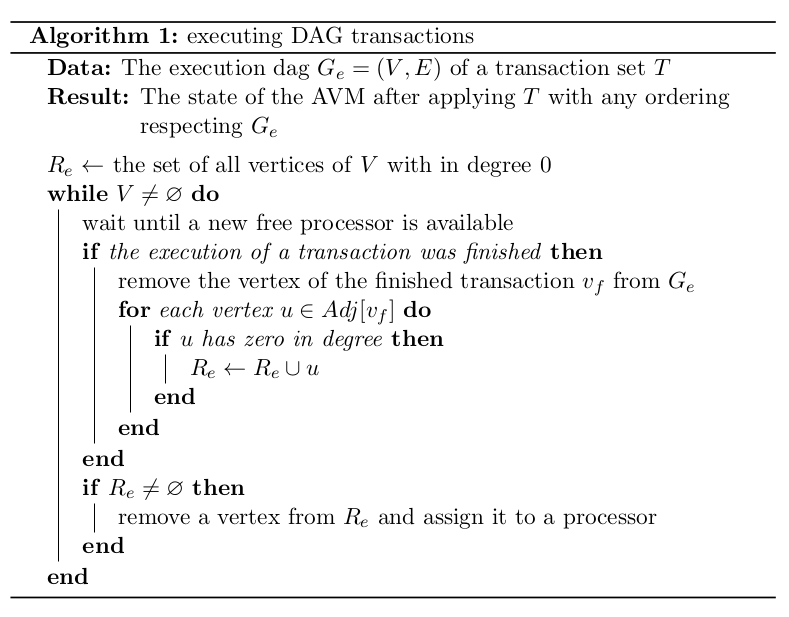
\includegraphics[width=17cm]{../img/Alg1s.png}
\begin{algorithm}[t]
    \DontPrintSemicolon
    \SetKwInOut{Input}{input}\SetKwInOut{Output}{output}
    \Input{A sequence of $n$ digits in base $\beta$: $d_{1}d_{2}\dots d_{n}$ \newline
    A prefix tree: $<0,A^{(1)},A^{(2)},A^{(3)},\dots>$}
    \BlankLine
    \Output{Valid identifier prefix of the sequence.}
    \BlankLine
    \For{$i = 1$ \KwTo $n$}
    {
        \If{$(0.d_{1}d_{2}\dots d_{i})_\beta < A^{(i)}$}
        {
            \KwRet{$d_{1}d_{2}\dots d_{i}$}\;
        }
    }
    \KwRet{NIL}\;
    \caption{Finding a prefixed identifier}\label{alg:prefix_id}
\end{algorithm}

When we have a prefixed identifier, and we want to know if a sequence of digits is marked by that identifier,
we use Algorithm~\ref{alg:match_id} to match the prefixed identifier with the start of the sequence. The matching
can be done with only three comparisons and an invalid prefixed identifier can also be detected.

In Argennon the shorter prefix codes are assigned to more active accounts and smart contracts which tend to own more
data objects in the system. The prefix trees are designed by analyzing empirical data to make sure the number
of leaves in each level is chosen appropriately.

\begin{algorithm}[h]
    \DontPrintSemicolon
    \SetKwData{Id}{$id$}
    \SetKwInOut{Input}{input}\SetKwInOut{Output}{output}
    \Input{A prefixed identifier in base $\beta$ with $n$ digits: $\Id=a_{1}a_{2}\dots a_{n}$ \newline
    A sequence of digits in base $\beta$: $d_{1}d_{2}d_{3}\dots $ \newline
    A prefix tree: $<0,A^{(1)},A^{(2)},A^{(3)},\dots>$
    }
    \BlankLine
    \Output{$TURE$ if and only if the identifier is valid and the sequence starts with the identifier.}
    \BlankLine
    \If{$(0.a_{1}\dots a_{n})_\beta = (0.d_{1}\dots d_{n})_\beta$}
    {
        \If{$A^{(n-1)} \leq (0.a_{1}a_{2}\dots a_{n})_\beta < A^{(n)}$}
        {
            \KwRet{TRUE}\;
        }
    }
    \KwRet{FALSE}\;
    \caption{Matching a prefixed identifier}\label{alg:match_id}
\end{algorithm}

\section{Arithmetics}\label{sec:arithmetics}

The Argennon Virtual Machine supports signed integer and signed floating point operations. The Argennon Virtual
Machine does not support any type of unsigned arithmetics. All arithmetic operations in the Argennon Virtual Machine
are checked and any type of overflow or underflow will cause a catchable exception to be thrown.

\section{Architecture}\label{sec:arch}


\subsection{The \texttt{pc} Register}\label{subsec:the-pc-register}

The Argennon Virtual Machine always has a single thread of execution and exactly has one \texttt{pc} register.
When the Argennon Virtual Machine is executing a method, if that method is not native, the \texttt{pc} register
contains the address of the AVM instruction currently being executed. If the method currently being executed
is native, the value of the Argennon Virtual Machine's \texttt{pc} register is undefined.

\subsection{Call Stack Queue}\label{subsec:call-stack}

Every AVM execution session has a queue of call stacks. A call stack contains all the information that is needed for
restoring the AVM's state and continuing the execution after the method invocation completes.
This information is represented by a \texttt{CallInfo} struct:
\begin{verbatim}
CallInfo {
    methodID,
    pc,
    localFrame,
    operandStack
} .
\end{verbatim}

The \texttt{methodID} field is the unique identifier of a method's bytecode that
is a composite prefix code built by concatenating an \texttt{applicationID} to
a local identifier.

Every method invocation has a corresponding \texttt{CallInfo} struct and when a method is invoked its
\texttt{CallInfo} struct is pushed onto the call stack. Hence, the top of the call stack always contains
the \texttt{CallInfo} struct of the current method. When a method invocation completes, its call
information is popped from the call stack.

An AVM execution session will continue as long as there is a non-empty call stack in the call stack queue. When the
execution of the current call stack finishes, the execution of the next call stack in the call stack queue starts.
It is possible that an AVM method invocation creates new call stacks. These newly created call stacks will be a part
of the current execution session and are added at the end of the call stack queue. A newly created call stack always
contains a single \texttt{CallInfo} struct. See Section~\ref{subsec:method-invocation} for more details.

\subsection{Run-Time Data Areas}\label{subsec:data-areas}

The Argennon Virtual Machine defines various run-time data areas that are used during an execution session,
Some of these data areas are persistent and are stored on the blockchain, Other data areas
are per execution session or per method invocation. These data areas are created when their context starts and
destroyed when their context ends.

The Argennon Virtual Machine has five run-time data areas:
\begin{itemize}
    \item Method Area
    \item Constant Area
    \item Local Frame
    \item Operand Stack
    \item Heap
\end{itemize}
All data areas except operand stack, have their own address space. Operand stack is a
last-in-first-out (LIFO) stack and is not addressable. Every AVM instruction operates on its specific
data areas.

\subsubsection{Method Area}

The method area contains the byte-code of any method which can be called by a non-native method invocation
instruction. In the Argennon Virtual Machine every method has a unique identifier:
\texttt{methodID}, and the method area is a map from method identifiers to their byte codes.

Every smart contract is required to have a special \texttt{dispatcher} method. The \texttt{dispatcher} method is the
only method of a smart contract that can be called by other smart contracts and has a
predefined \texttt{methodID}: \texttt{(ApplicationID|0)}.

\note{The Argennon Virtual Machine does not have internal or external methods. All methods are considered internal
except the \texttt{dispatcher} method, which is the only external method of any smart contract.
This design enables the AVM to execute \emph{RESTful} smart contracts more efficiently.}

Instructions that modify the code area can only be run in privileged mode, which means they can only be executed
by the \emph{root} smart contract. As a result, the access of smart contracts to the code area is essentially
read-only.

\subsubsection{Constant Area}

Every smart contract has a single constant area which is stored in the AVM code area as a special type of
non-executable method. The constant area of a smart contract contains user
defined constants.

\note{Instructions that modify the constant area can only be run in privileged mode.}


\subsubsection{Local Frame}

A local frame is used to store methods parameters and local variables. A new frame is created each time a method
is invoked, and it is destroyed when its method invocation completes, whether the completion is normal or abrupt.

\subsubsection{Operand Stack}

Every time a local frame is created, a corresponding empty last-in-first-out (LIFO) stack is created too. The
Argennon Virtual Machine is a stack machine and its instructions take operands from the operand stack, operate on
them, and push the result back onto the operand stack. An operand stack is destroyed when its owner method
completes, whether that completion is normal or abrupt.

\subsubsection{Heap}

The heap of the Argennon Virtual Machine is a persistent memory area which stores \emph{memory chunks}. A Memory
chunk is a byte addressable piece of continuous memory which has a separate address space starting from 0. Each chunk
has a fixed size and different chunks need not be equally sized. Chunks are stored in the heap area and every chunk is
assigned a unique identifier: \texttt{chunkID}. As a result, the address of every memory location inside
the heap area can be considered as a pair: \texttt{(chunkID, offset)}.

A smart contract can read any chunk stored in the heap by having its \texttt{chunkID}. However, it can only modify
those chunks that was created by itself. In other words, every memory chunk in the AVM's heap has an owner. Only
the owner can modify a chunk while anyone can read that chunk. The owner of a chunk can be easily determined
by the \texttt{applicationID} part of the chunk identifier.

\note{The reason behind this type of access control design is the fact that smart contract code is usually
immutable. That means if a smart contract does not implement a getter mechanism for some parts of its internal
data, this functionality can never be added later, and despite the internal data is publicly available, there will
be no way for other smart contracts to use this data on-chain. This design eliminates the need for implementing
\emph{trivial} getters.}

The AVM Heap is able to save snapshots of its state and later restore them. This will enable the Argennon
Virtual Machine to have state reversion capability. The snapshot management of the heap area is done by
the following functions:
\begin{itemize}
    \item \texttt{Save()} saves a snapshot of the current state of the heap and pushes it onto the
    snapshot stack.
    \item \texttt{Restore()} pops the snapshot stored on the top of the snapshot stack and restores it. The
    current state of the heap will be lost.
    \item \texttt{Discard()} pops the snapshot stored on the top of the snapshot stack and discards it. The current
    state of the heap will not change.
\end{itemize}

\note{These functions are internal functions of the AVM. They are not instructions, and can not be called by smart
contracts.}

\section{Instruction Set Overview}\label{sec:instruction-set-overview}

An Argennon Virtual Machine instruction consists of a \textbf{one-byte} opcode specifying the operation to be
performed, followed by zero or more operands supplying arguments or data that are used by the operation.
The number and size of the operands are determined solely by the opcode.

\subsection{Method Invocation}\label{subsec:method-invocation}

The Argennon Virtual Machine has four types of method invocation instruction:
\begin{itemize}
    \item \texttt{invoke\_internal}: invokes a method without changing the context of method execution. In other
    words, the invoked method can only modify the state of the current smart contract.
    A smart contract can invoke any method by \texttt{invoke\_internal} instruction, even if that method is an
    internal method of another smart contract. Since the invoked method will always be executed in the context of
    the invoking smart contract, a smart contract will not be able to modify another smart contract's state by
    this instruction. This instruction facilitates code reuse and the usage of libraries.
    If the invoked method completes abruptly, the invoker method completes abruptly too.
    \item \texttt{invoke\_dispatcher}: invokes the \texttt{dispatcher} method of a smart contract and changes the
    context of method execution to that
    smart contract. If the invoked method completes abruptly, that will cause the invoker method to complete
    abruptly too.
    \item \texttt{i\_invoke\_dispatcher, i\_invoke\_internal}: independently invokes a method. These instructions
    are similar to their \texttt{invoke} counterparts, with the difference that when
    the invoked method completes abruptly, the invoker method can continue execution. When a method invoked by
    an \texttt{i\_invoke} instruction completes abruptly, all changes made
    by the invoked method to the AVM's state will be reverted and the instruction will act like
    a jump to the specified error handling code.
    \item \texttt{invoke\_native}: invokes a method that is not hosted by the Argennon Virtual Machine. By this
    instruction, high performance native methods of the hosting machine, such as GPU accelerated operations,
    could become available to AVM smart contracts. This instruction will not modify the AVM's state.
    \item \texttt{invoke\_later}: invokes the \texttt{dispatcher} method of another smart contract by creating a new
    call stack. The created call stack is added at the end of the call stack queue, and
    the context of method execution will change after the execution of that call stack starts. This instruction does
    not modify the \texttt{pc} register and the execution of the
    invoker will continue after this instruction. As a result, \texttt{invoke\_later} can not return
    any values to the caller and the return value of the called method (if any) will be discarded. If the invoked
    method completes abruptly, it will cause \textbf{all the call stack queue to
    complete abruptly.}
\end{itemize}

\note{The \texttt{invoke\_later} instruction can be used to call a smart contract while its reentracy lock is active.
Because the invocation uses a separate call stack, it will not cause the lock to throw an exception.}

Each time a method is invoked a new local frame
and operand stack is created. If the method was invoked by an \texttt{i\_invoke} instruction,
the \texttt{Save()} function of the AVM's heap is called before the execution of the method starts.

The Argennon Virtual Machine uses local frames to pass parameters on
method invocation. On method invocation, any parameters are passed in consecutive local variables stored in the
method's local frame starting from address 0. The invoker of a method writes the parameters in the local frame
of the invoked method using \texttt{arg} instructions.

\note{The AVM does not natively support polymorphism and virtual methods. A compiler could easily
generate appropriate code for implementing these features.}

\subsection{Exceptions}\label{subsec:exceptions}

An exception is thrown programmatically using the \texttt{athrow} instruction. Exceptions can also be thrown by
various Argennon Virtual Machine instructions if they detect an abnormal condition.

\note{Any AVM instruction may throw an exception. This happens when the execution cost of a transaction has exceeded
the declared maximum execution cost.}

\subsection{Method Invocation Completion}\label{subsec:method-invocation-completion}

A method invocation completes normally if that invocation does not cause an exception to be thrown, either
directly from the AVM or as a result of executing an explicit throw statement. If the invocation of the current
method completes normally and the invocation was not made by an \texttt{invoke\_later} instruction, then a value may be
returned to the invoking method. This occurs when the invoked method executes one of the return instructions, the
choice of which must be appropriate for the type of the value being returned (if any). Execution then continues
normally in the invoking method's local frame with the returned
value (if any) pushed onto the operand stack. If the method was invoked by an \texttt{invoke\_later} instruction,
the execution of the next call stack (if any) begins and the returned value
is discarded. When a method invocation that was made by
an \texttt{i\_invoke} instruction completes normally,
the \texttt{Heap.Discard()} function is called as a part of the return instruction.

A method invocation completes abruptly when an exception is thrown by one its instructions.
The \texttt{invoke\_internal} and \texttt{invoke\_dispatcher} instructions
always throw an exception when their invoked method completes abruptly. A
method invocation that completes abruptly never returns a value.

When a method completes normally, the call stack is used to restore the state of the invoker,
including its local frame and operand stack, with the \texttt{pc} register appropriately restored and incremented
to skip past the method invocation instruction. If the current call stack is empty the next call stack in the call
stack queue will be used for continuing the execution, and when there are no call stacks left in the queue the
current execution session ends.

When a method completes abruptly, the call stack is used to restore the \texttt{pc} register of the invoker. If the pc
register points to an \texttt{invoke} instruction, the current method completes abruptly as well. Otherwise, if
the \texttt{pc} register is pointing to an \texttt{i\_invoke} instruction, the \texttt{Heap.Restore()} function is
called to restore the state of the AVM's heap. Then, the
local frame and operand stack of the invoker is restored, and execution continues after branching to the error handling
code specified by the instruction's operand.

When an invocation which was made by an \texttt{invoke\_later} instruction completes abruptly, the
heap snapshot that was saved before the start of the
execution of the first call stack is restored. This means
that all changes made by the execution session to the AVM's heap will be completely reverted.

\subsection{Reentrancy Protection}\label{subsec:reentrancy}

The Argennon Virtual Machine provides low level reentrancy protection by defining a dedicated
instruction: \texttt{enter}. When a smart contract executes the \texttt{enter} instruction, it
can not execute that instruction again as long
as the method executing the instruction completes (abruptly or normally). If a smart contract tries to execute
the \texttt{enter} instruction while the method executing that instruction for the first time has not yet completed,
an exception will be thrown.

Smart contracts can completely prevent reentrancy by executing the \texttt{enter} instruction as the first instruction
of their \texttt{dispatcher} method.

\subsection{Heap Allocation and Deallocation}\label{subsec:heap-allocation-instructions}

Heap allocation and deallocation in the Argennon Virtual Machine is done by the following instructions:

\begin{itemize}
    \item \texttt{alloc}: creates a new memory chunk of the specified size in the heap. The
    new chunk's identifier will be the concatenation of the \texttt{applicationID} of the creator of the chunk and
    the \texttt{id} operand of the instruction. The \texttt{id} operand must be the concatenation of
    an \texttt{accountID} and a prefix code
    generated by the \emph{local} prefix tree: \texttt{id = accountID|localID}. If the identifier is not valid or
    if it already exists in the heap, a catchable exception will be thrown.

    \item \texttt{delete}: deletes the chunk that its identifier is the concatenation of the current smart
    contract \texttt{applicationID} and the specified \texttt{id} operand. If the identifier is not valid or
    if the chunk was not found, a catchable exception will be thrown.
\end{itemize}

When a smart contract allocates a new memory chunk, the identifier of the new chunk is not generated by
the AVM. Instead, the smart contract can choose an identifier itself. This is a very important feature of
the AVM's heap, which allows smart contracts to use the AVM's heap as a dictionary (map) data structure.
Since the \texttt{chunkID} is a prefix code, any smart contract has its own identifier space, and a smart contract
can easily generate unique identifiers for its chunks.

The AVM requires the chosen identifier to be a prefix code compatible with
the \emph{accounts} prefix tree, or a code made by concatenating a code compatible with
the \emph{accounts} prefix tree to a code compatible with the \emph{local} prefix tree. This requirement
enables AVM to detect invalid identifiers, while smart contracts can easily associate data with account identifiers.
At the same time, A smart contract is able to create maps with costume keys by appending local identifiers
to the zero \texttt{accountID}. Zero \texttt{accountID} does not correspond to a valid account in the Argennon
blockchain.


\section{Authorizing Operations}\label{sec:authorizing-operations}

In blockchain applications, we usually need to authorize certain operations. For example, for sending an asset
from a user to another user, first we need to make sure that the sender has authorized this operation. The
Argennon Virtual Machine has no built-in mechanism for authorizing operations, but it provides a rich set of
cryptographic instructions for validating signatures and cryptographic entities. By using these instructions and
passing cryptographic signatures as parameters to methods, a programmer, having users' public keys, can implement
the required logic for authorizing any operation.

\note{Authorization by explicit signatures eliminates the need for approval methods or call back patterns.}

In addition to cryptographic signatures, the Argennon Virtual Machine provides instructions that enable
smart contracts to issue \emph{virtual signatures}. A smart contract can virtually sign a message for a target
smart contract by \texttt{v\_sign} instruction. When a smart contract
virtually signs a message for a target, that message is stored in the internal memory of the AVM, associated with
its signer and the target. The application that is the target of the signature can verify the message
by \texttt{v\_verify} instruction. After verifying the signature, it will be removed from the AVM's internal memory
to make sure a signature will not be used multiple times. The virtual signatures stored in the AVM's internal memory
last for one execution session.

\note{The Argennon virtual machine has no instructions for issuing cryptographic signatures.}


\section{The AVM Standard Library}\label{sec:the-avm-standard-library}

As we explained in Section~\ref{subsec:method-invocation} by using \texttt{invoke\_internal} instruction, a smart
contract can invoke methods of another smart contract in its own context. AVM smart contracts use this instruction to
invoke methods of the AVM standard library. Methods of the AVM standard library are stored
with the \texttt{applicationID} zero in the AVM method area. This implies that the AVM standard library is actually
a part of the root smart contract.

In Argennon, the root smart contract is an updatable smart contract, which can be updated by the Argennon governance
system. This means that bugs or security vulnerabilities in the AVM standard library could be quickly patched and
smart contracts could benefit from bugfixes and improvements of the AVM standard library even if they are
non-updatable. Many important and useful functionalities,
such as fungible and non-fungible assets, access control mechanisms,
and general purpose DAOs are implemented in the Argennon standard library.

All Argennon standards, for instance ARC standard series, which defines standards regarding transferable assets,
are defined based on how a contract should use the AVM standard library. As a result, Argennon standards are
different from conventional blockchain standards. Argennon standards define some type of standard logic and
behaviour for a smart contract, not only a set of method signatures. This enables users to expect certain type
of behaviour from a contract which complies with an Argennon standard.
